%%==================================================================%%
%% Author : Tejedo Gonz�lez, Daniel                                 %%
%%          S�nchez Barreiro, Pablo                                 %%
%% Version: 1.0, 18/11/2012                                         %%                   
%% Version: 1.0, 06/02/2013                                         %%                   
%%                                                                  %%
%% Memoria del Proyecto Fin de Carrera                              %%
%% Antecedentes, arquitectura de plugins de eclipse                 %%
%%==================================================================%%

El entorno de desarrollo Eclipse es un ejemplo de arquitectura modular f�cilmente extensible mediante una compleja, pero sencilla al programador, arquitectura de \emph{plug-ins}. Un \emph{plug-in} en Eclipse es un componente que provee un cierto tipo de servicio dentro del contexto del espacio de trabajo de Eclipse. Es decir, una herramienta que se puede integrar en el entorno Eclipse junto con sus otras funcionalidades. Dado que la herramienta \emph{Hydra} fue dise�ada como un \emph{plug-in} para Eclipse, y nuestro editor pretende integrarse tanto en \emph{Hydra} como en \emph{Eclipse}, es necesario conocer y manejar el funcionamiento de la arquitectura de plug-ins de Eclipse.

Aunque la arquitectura de plug-ins de Eclipse tiene mucha profundidad y ofrece muchas posibilidades, es imprescindible el dominio de dos de sus conceptos clave para poder trabajar con ella: las dependencias y los puntos de extensi�n.  Mediante las dependencias podemos indicar que el plug-in a desarrollar tiene que incorporar toda la funcionalidad y estructura de otro plug-in (en este caso nuestro editor tiene, entre otras, una dependencia con el plug-in de la herramienta Hydra original). Un punto de extensi�n permite a�adir cierta funcionalidad al plug-in desarrollado mediante la inclusi�n autom�tica de ciertos segmentos de c�digo. Un ejemplo cl�sico de punto de extensi�n, y que adem�s ha sido utilizado en el transcurso de este proyecto, es el que permite a�adir un bot�n a la barra de tareas de Eclipse de manera autom�tica, teniendo que implementar �nicamente el c�digo del manejador de ese bot�n.

 \begin{figure}[!tb]
    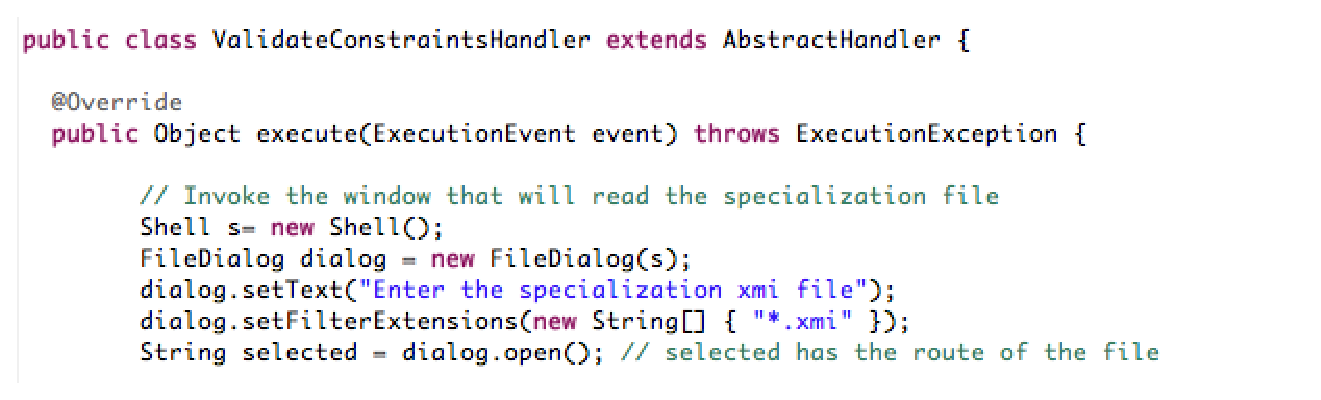
\includegraphics[scale=0.4]{background/codigoManejador.eps}
    \caption{Trozo de c�digo del manejador de un bot�n introducido mediante un punto de extensi�n}
    \label{fig:codigoManejador}
\end{figure}

%%==============================================================================================%%
%% NOTA(Pablo): Esto no se entiende nada
%%==============================================================================================%%
%%
%% En particular, se han utilizado mucho los puntos de extensi�n. Un punto de extensi�n en un
%% plug-in indica la posibilidad de que ese plug-in sea a su vez parte de otro, o que haya 
%% otros plug-ins que sean parte de �l. Esta particularidad permite no s�lo la integraci�n de 
%% nuestro editor con Hydra, sino tambi�n la personalizaci�n de men�s y botones para �l 
%% gracias a la creaci�n de puntos de extensi�n con plug-ins de creaci�n de men�s y barras de
%% herramientas.
%%
%%==============================================================================================%%

%%==============================================================================================%%
%% NOTA(Pablo): Para solucionar
%% - Describir en uno o dos p�rrafos c�mo funciona la arquietctura de plug-ins para Eclipse
%% - Poner un ejemplo de punto de extensi�n, sencillo y concreto, y explicar como funciona 
%%   el punto de extensi�n utilizando algo de c�digo.
%% Si no sabes como escribir esta secci�n, la eliminas directamente, y actualizas la intro 
%% al Cap�tulo de forma conveniente.
%%==============================================================================================%%
